\documentclass{beamer}
\mode<presentation>
\usetheme{CambridgeUS}
\usepackage[russian]{babel}
\usepackage[utf8]{inputenc}
\usepackage[T2A]{fontenc}
\usepackage{sansmathaccent}
\pdfmapfile{+sansmathaccent.map}
\title[Восприятие звука]{Восприятие звука человеком, элементы психофизиологической акустики}
\author{Наумов Д.А.}
\date[16.02.2014] {Компьютерные музыкальные технологии и звуковой дизайн, 2014}

\begin{document}

%ТИТУЛЬНЫЙ СЛАЙД
\begin{frame}
  \titlepage
\end{frame}
  
%СОДЕРЖАНИЕ ЛЕКЦИИ
\begin{frame}
  \frametitle{Содержание лекции}
  \tableofcontents  
\end{frame}
  
%РАЗДЕЛ 1
\section[Элементы психофизиологической акустики]{Восприятие звука человеком, элементы психофизиологической акустики}
\begin{frame}
{\itshape Акустика} (от греч. "<akustikos">~--- слуховой)~--- область физики, изучающая возникновение, распространение и взаимодействие с веществом звуковых волн от самых низких частот до самых высоких.
{\itshape Психофизиологическая акустика}~--- наука, изучающая психологические и физиологические особенности восприятия звука человеком. Основные задачи психофизиологической акустики являются: 
\begin{itemize}
\item исследование влияния звука на человека;
\item исследование процесса получения и обработки звуковой информации мозгом человека;
\item выработка правил, норм и рекомендаций по нейтрализации вредного влияния звука на человека при нахождении его в звуковой среде, а также при использовании различной звуковой аппаратуры и приборов.
\end{itemize} 
\end{frame}   

\begin{frame}
\section{Слуховой аппарат человека}
\begin{figure}
\centering
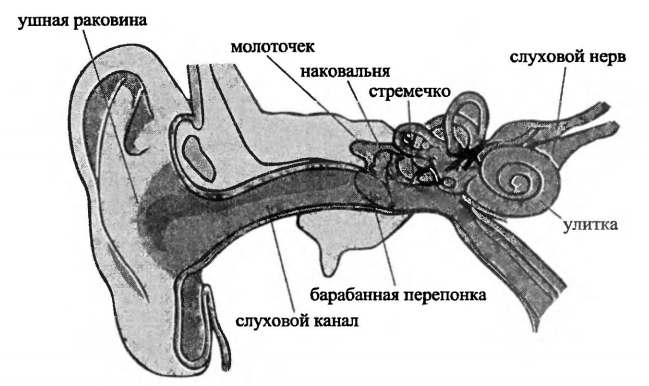
\includegraphics[width=0.9\linewidth]{pic-ear-01}
\end{figure}
Звуковые колебания воспринимаются по двум принципам:
\begin{itemize}
\item ударному: до $400$~Гц $\rightarrow$ $4000$~Гц;
\item частотному: свыше $4000$~Гц.
\end{itemize}
\end{frame}

\begin{frame}
Слуховой аппарат человека способен различать частотные составляющие звука приблизительно в пределах от 20-30 Гц до 20 кГц (слышимый звук).  Частоты ниже~---инфразвук, выше~---ультразвук.
\begin{figure}
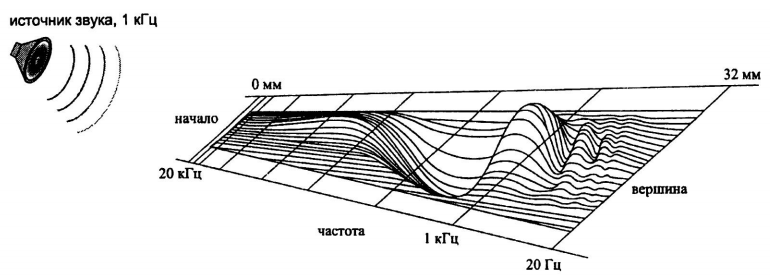
\includegraphics[width=0.9\linewidth]{pic-ear-02}
\end{figure}
Базилярная мембрана $\approx$ набор слуховых полосно-пропускающих фильтров, расположенных в определенном порядке (по частоте убывания от 20 кГц до 20 Гц) с определенной величиной перекрытия, покрывающих всю полосу слышимых частот. 

Ширина слухового фильтра составляет приблизительно 10-20\% от его центральной частоты.
\end{frame}

\begin{frame}
Пример. Ширина фильтра с центральной частотой 13,5 кГц составляет приблизительно 3,5 кГц. 

Зависимость ширины слуховых фильтров от их центральной частоты:
\begin{figure}
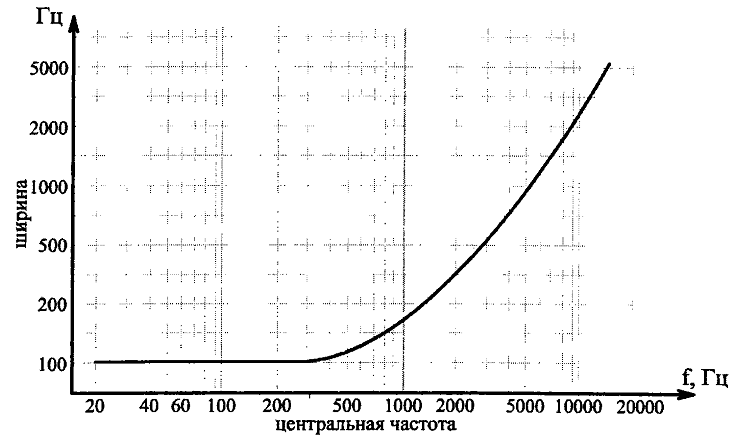
\includegraphics[width=0.9\linewidth]{pic-ear-03}
\end{figure}
\end{frame}

\begin{frame}
Критическая полоса~--- это минимальная полоса частот, которая возбуждает одну и ту же часть базилярной мембраны. 
\begin{itemize}
\item В частотном промежутке от 0 до 16 кГц опытным путем были определены 24 критические полосы. 
\item Звуковой сигнал в пределах одной и той же критической полосы как бы обобщается мозгом, создавая близкие слуховые ощущения.
\item На "<распознавание"> высокочастотных сигналов на мембране отведено меньше площади поверхности, чем на распознавание низких частот. 
\begin{enumerate}
\item Высокие частоты менее важны для человека, чем низкие.
\item Длина мембраны ограничена 32 мм, а для определения низкочастотных колебаний требуется большая площадь, чем для определения высокочастотных из-за существенной разницы длин волн. \end{enumerate}
\end{itemize}
Следствие: человек легче (увереннее) распознает изменения в полосе низких частот, чем в полосе высоких.
\end{frame}

\begin{frame}
\begin{table}[h!]
  \caption{Критические полосы и соответствующие им параметры}
  \begin{center}
  \begin{tabular}{|p{0.10\textwidth}|p{0.20\textwidth}|p{0.20\textwidth}|p{0.20\textwidth}|}
  \hline Номер полосы, Барк & Критическая полоса, Гц & Ширина критической полосы, Гц & Центральная частота критической полосы, Гц \\
  \hline 0 & \centering 0 - 0 & \centering 100 & 50 \\
  \hline 1 & \centering 100 - 200 &\centering 100 & 150 \\
  \hline 2 & \centering 200 - 300 &\centering 100 & 250 \\
  \hline 3 & \centering 300 - 400 &\centering 100 & 350 \\
  \hline 4 & \centering 400 - 510 &\centering 110 & 450 \\
  \hline 5 & \centering 510 - 630 &\centering 120 & 570 \\
  \hline 6 & \centering 630 - 770 &\centering 140 & 700 \\
  \hline 7 & \centering 770 - 920 &\centering 150 & 840 \\
  \hline 8 & \centering 920 - 1080 &\centering 160 & 1000 \\
  \hline 9 & \centering 1080 - 1270 &\centering 190 & 1170 \\
  \hline 10 & \centering 1270 - 1480 &\centering 210 & 1370 \\
  \hline
  \end{tabular}  
  \end{center}  
\end{table}
\end{frame}

\begin{frame}
\begin{table}[h!]
  \begin{center}
  \begin{tabular}{|p{0.10\textwidth}|p{0.20\textwidth}|p{0.20\textwidth}|p{0.20\textwidth}|}
  \hline Номер полосы, Барк & Критическая полоса, Гц & Ширина критической полосы, Гц & Центральная частота критической полосы, Гц \\
  \hline 11 & \centering 1480 - 1720 &\centering 240 & 1600 \\
  \hline 12 & \centering 1720 - 2000 &\centering 280 & 1850 \\
  \hline 13 & \centering 2000 - 2310 &\centering 320 & 2150 \\
  \hline 14 & \centering 2320 - 2700 &\centering 380 & 2500 \\
  \hline 15 & \centering 2700 - 3150 &\centering 450 & 2900 \\
  \hline 16 & \centering 3150 - 3700 &\centering 550 & 3400 \\
  \hline 17 & \centering 3700 - 4400 &\centering 700 & 4000 \\
  \hline 18 & \centering 4400 - 5300 &\centering 900 & 4800 \\
  \hline 19 & \centering 5300 - 6400 &\centering 1100 & 5800 \\
  \hline 20 & \centering 6400 - 7700 &\centering 1300 & 7000 \\
  \hline 21 & \centering 7700 - 9500 &\centering 1800 & 8500 \\
  \hline 22 & \centering 9500 - 12000 &\centering 2500 & 10500 \\
  \hline 23 & \centering 12000 - 15500 &\centering 3500 & 13500 \\
  \hline
  \end{tabular}  
  \end{center}  
  \label{tab-crit-01}
\end{table}
\end{frame}

\section{Психофизиологические акустические параметры звука}
\subsection{Тон, высота тона и тембр звука}

\begin{frame}
  \begin{block}{Основная частота (тон)}
    наиболее выделяющаяся по амплитуде и периоду частотная составляющая.   
  \end{block}

  \begin{block}{Обертона}
    тоны, соответствующие остальным частотам спектра. Если частоты обертонов кратны   частоте основного тона, то обертоны называют {\itshape гармониками}, а основной тон~---{\itshape первой гармоникой}
  \end{block}

Для периодических сигналов слуховая система человека способна различать высоту звука.

  \begin{block}{Высота звука}
    характеристика, условно распределяющая звуки по некоторой шкале от низких к высоким.
  \end{block}

На воспринимаемую высоту звука влияет, главным образом, частота основного тона, однако форма периода звуковой волны и ее состав также могут оказывать влияние на высоту звука.

\end{frame}

\begin{frame}
В зависимости от соотношения амплитуд частотных составляющих спектра, звук может приобретать различную окраску и восприниматься, как {\itshape тон} или как
{\itshape шум}. 

\begin{itemize}
\item Дискретный спектр, один максимумум $\rightarrow$ тон;
\item Дискретный спектр, один несколько максимумов $\rightarrow$ созвучие;
\item Сплошной спектр $\rightarrow$ шум.
\end{itemize}

{\itshape Высота тона}~--- это субъективная характеристика ощущения физической частоты тона.

Частотная разрешающая способность слуха ухудшается при переходе от нижних частот к верхним: 
\begin{itemize}
\item от 0 до 16 кГц до 620 градаций частот;
\item от 0 до 500 Гц до 140 градаций частот.
\end{itemize}

На восприятии высоты звука чистых тонов сказываются:
\begin{itemize}
\item интенсивность звучания;
\item длительность звучания. 
\end{itemize}
Низкий чистый тон кажется более низким при увеличении интенсивности. 
Высокий чистый тон кажется более высоким при увеличении интенсивности.
\end{frame}

\begin{frame}
\begin{block}{Мел}
("<melody">~--- "<мелодия">)~--- единица измерения ощущения высоты тона. 
\end{block}

Равное изменение частоты в мелах соответствует равному изменению ощущения высоты тона. 

~

Интервалы от 500 до 1000~Гц и от 1000 до 2000 Гц $\rightarrow$ неравные. 
Интервалы от 500 до 1000~мел и от 1000 до 2000 мел $\rightarrow$ равные. 

~

Эмпирическая формула перевода герц в мелы выглядит следующим образом:
\[ m[\text{мел}]=1127,01048 \log_{10}(1+\frac{f[\text{Гц}]}{700}),\]
где \(f\)~--- частота, измеренная в герцах, \(m\)~--- частота, измеренная в мелах.
\end{frame}

\begin{frame}
\begin{block}{График соотношения между шкалами герц и мелов}
\centering{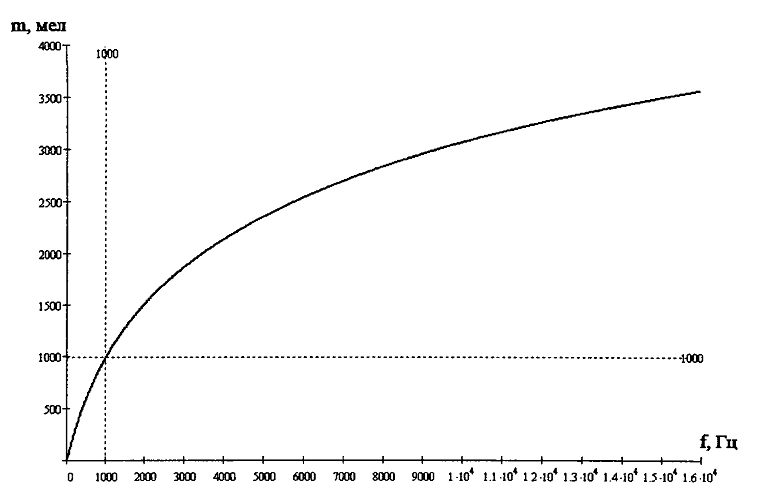
\includegraphics[width=0.8\linewidth]{pic-ear-04}}
\end{block}
\end{frame}

\begin{frame}
Мел и Барк~--- психофизиологические акустические единицы измерения высоты тона, используемые в психоакустике при оценке субъективной высотой тона. 
\begin{block}{График соотношения трех шкал}
\centering{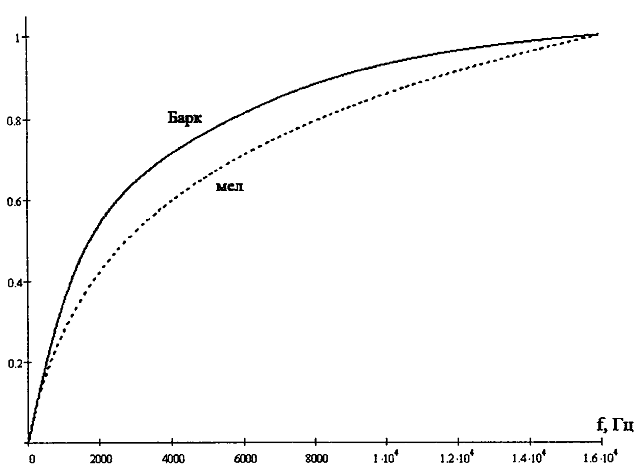
\includegraphics[width=0.7\linewidth]{pic-ear-05}}
\end{block}
\end{frame}

\begin{frame}
  \begin{block}{Тембр звука}
качество звука, которое, вне зависимости от частоты и амплитуды, позволяет отличить одно звучание от другого. 
  \end{block}

  Тембр звука:
  \begin{enumerate}
    \item зависит от общего спектрального состава звука;
    \item зависит от соотношения амплитуд составляющих спектра
    \item фактически не зависит от высоты основного тона.
  \end{enumerate}  

  ~

  Тембр звука с одним и тем же основным тоном определяется составом обертонов (их частотами и амплитудами), а также характером нарастания амплитуд в начале звучания и их спадания в конце звучания. 
  ~  
  На распознавание тембра слуховой системе требуется около 200 мс. 
\end{frame}

\begin{frame}
  \begin{block}{Сигналограммы звучания трубы и фортепиано ноты "<ля"> первой октавы}
    \centering{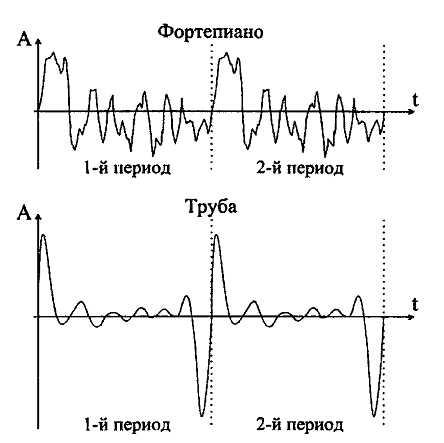
\includegraphics[width=0.6\linewidth]{pic-ear-06}}
  \end{block}
  Высота тона у обоих сигналов одинакова и определяется периодом колебаний. 
\end{frame}

\subsection{Интенсивность и громкость звука}
\begin{frame}
  Уровень громкости звука является функцией его интенсивности и частоты. 

  \begin{block}{Интенсивностью (силой) звука} 
  называется количество звуковой энергии $W_\text{з}$ переносимой звуковой волной за единицу времени $t$ через единицу площади поверхности $S$, нормальной к направлению распространения звуковой волны:
\[I=\frac{W_\text{з}}{St}=\frac{N_\text{з}}{t}\, \text{Вт}/\text{м}^2\]
где $N_\text{з}$~--- звуковая мощность, Вт; $W_\text{з}$~--- звуковая энергия, Дж; $S$~--- площадь поверхности, перпендикулярной к направлению распространения звуковой волны (звука), $m^2$.
  \end{block}

  \begin{block}{Громкость звука}
  это психофизиологическая характеристика восприятия звука, определяющая ощущение интенсивности (силы звука), т.е. {\itshape громкость звука является мерой силы слухового ощущения}. 
  \end{block}
 
\end{frame}

\begin{frame}
Громкость звука нарастает непропорционально увеличению интенсивности сигнала. 
\begin{block}{Закон Вебера-Фехнера}
прирост силы ощущения пропорционален логарифму отношения интенсивностей двух сравниваемых раздражений.
\end{block}

Величина, оценивающая громкость звука,~--- это уровень интенсивности звука $L_I$ который определяется соотношением

\[L_I=k \log_{10}{\frac{I}{I_0}}, \text{дБ}\]
где $I$~--- измеряемая интенсивность (сила) звука, $\text{Вт}/\text{м}^2$; $I_0\approx 10^{-12} \text{Вт}/\text{м}^2$~--- интенсивность самого слабого звука, воспринимаемого человеческим ухом, принятая за {\itshape порог интенсивности} (т.е. за нижний предел чувствительности (слышимости) человеческого уха); $k$~--- коэффициент пропорциональности: при $k=1$ уровень звука выражается в белах, при $k=10$ уровень звука выражается в децибелах.
\end{frame}

\begin{frame}
Эффективное звуковое давление может быть рассчитано по следующей формуле:
\[P_{\text{эф}}=\sqrt{I \rho C}.\]

Величину \(P_{0~\text{эф}}=2\cdot10^{-5}\ \text{Н}/\text{м}^2\) называют порогом звукового давления; это наименьшая величина эффективного звукового давления, соответствующая порогу интенсивности $I_0$.

\begin{block}{Порог слышимости}
наименьшее значение величины эффективного звукового давления, при котором звук еще воспринимается органами слуха. 
\end{block}
Порог слышимости также зависит от частоты звука и может достигать своего минимального значения в широком диапазоне частот ($700-6000$ Гц). Поэтому принят так называемый стандартный порог слышимости, соответствующий частоте $f=1000$ Гц.
\end{frame}
 

\begin{frame}
\begin{block}{Приблизительные значения уровней громкости звуков}
\centering{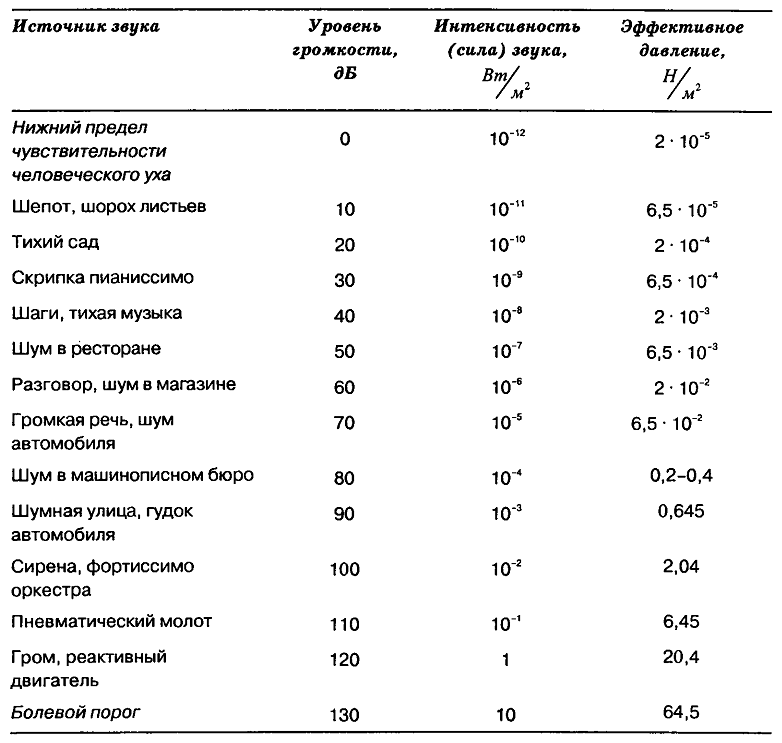
\includegraphics[width=0.7\linewidth]{pic-ear-07}}
\end{block}
\end{frame} 

\begin{frame}
\begin{block}{Кривые равной громкости}
\centering{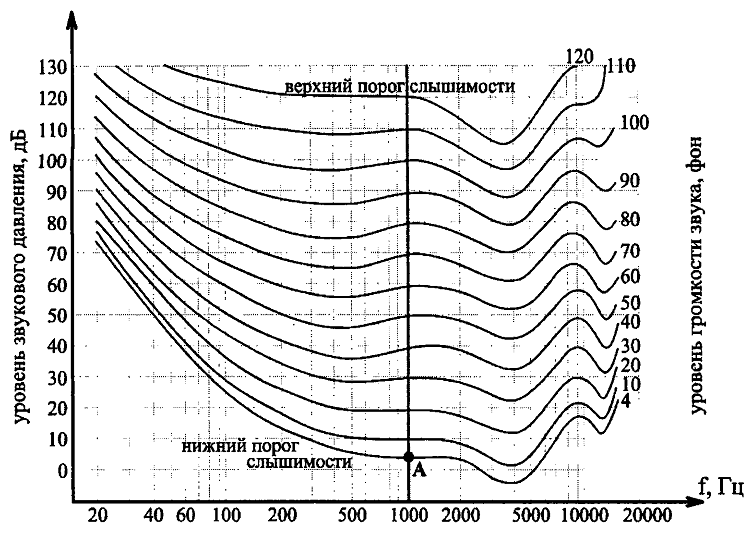
\includegraphics[width=0.7\linewidth]{pic-ear-08}}
\end{block}
Под одним {\itshape фоном} (от англ. "<рhon">) следует понимать уровень громкости звука, для которого уровень звукового давления равногромкого с ним звука частоты 1000 Гц равен 1 дБ. 
\end{frame} 

\subsection{Порог слышимости и маскировка}
\begin{frame}
  \begin{block}{График порога слышимости для различных возрастов слушателя}
    \centering{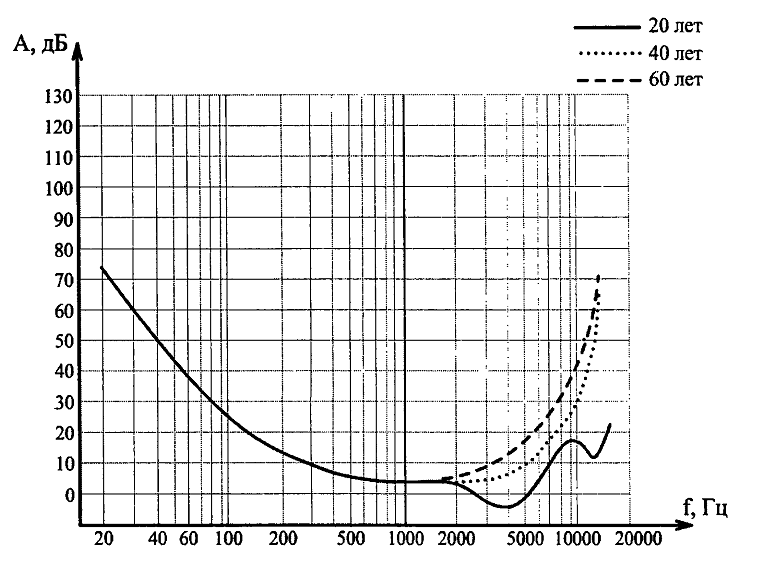
\includegraphics[width=0.8\linewidth]{pic-ear-10}}
  \end{block}
\end{frame}

\begin{frame}
  \begin{block}{Диаграмма слуховых ощущений}
    \centering{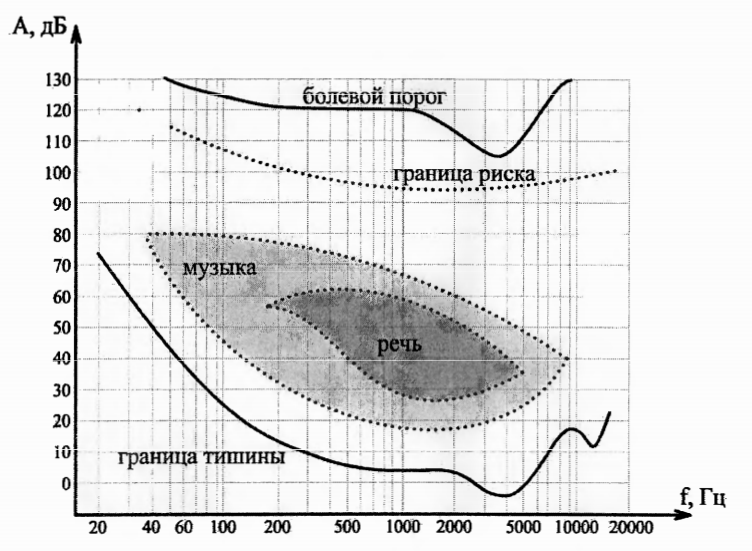
\includegraphics[width=0.8\linewidth]{pic-ear-11}}
  \end{block}
\end{frame}

\begin{frame}
  \begin{block}{Диаграмма частотной маскировки}
    \centering{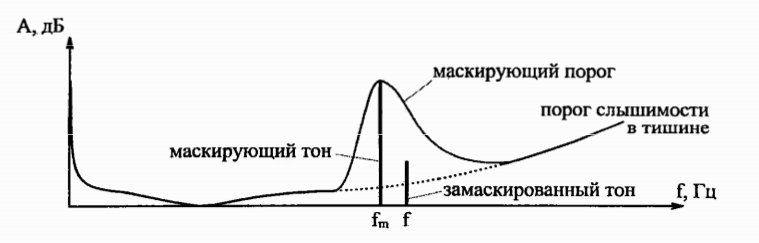
\includegraphics[width=0.8\linewidth]{pic-ear-12}}
  \end{block}
  \begin{block}{Диаграмма временн{\'o}й маскировки}
    \centering{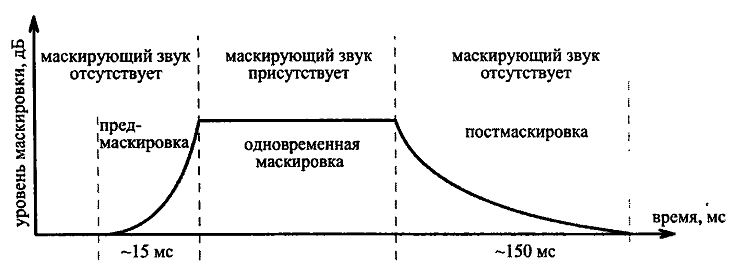
\includegraphics[width=0.8\linewidth]{pic-ear-13}}
  \end{block}  
\end{frame}
 
\section{Восприятие пространственности звука} 
\begin{frame}
  Слуховой аппарат человека способен определить направление звукового сигнала:
  \begin{itemize}
    \item по разнице во времени попадания сигнала в левое и правое ухо в пределах до 1 мс ($300-1000$~Гц). 
    \item путем анализа громкости звука (выше 1000~Гц).
  \end{itemize} 
  \centering{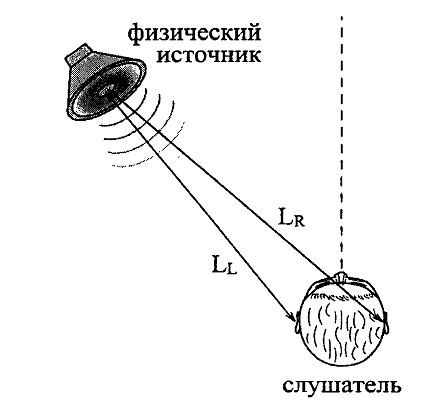
\includegraphics[width=0.6\linewidth]{pic-ear-14}}
\end{frame} 
 
\begin{frame}
  \begin{block}{Стереофония} 
    донесение до слушателя пространственного звучания.
  \end{block}
  \begin{block}{Стереобаза} 
    мнимая линия, соединяющая два физических источника звука при воспроизведении звукового сигнала, на которой располагаются мнимые источники звука.
  \end{block}
  \centering{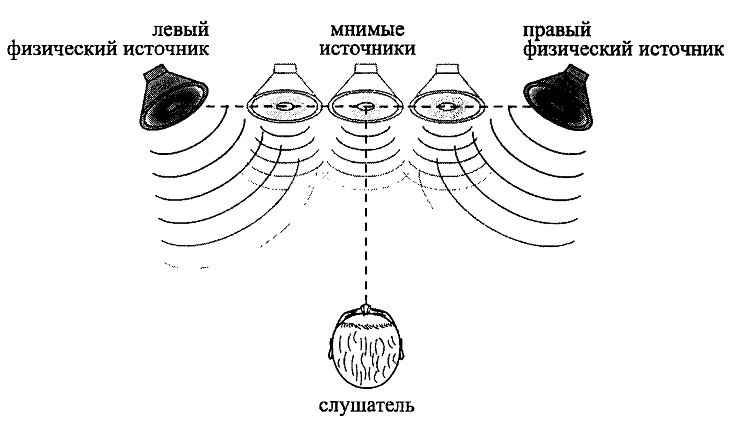
\includegraphics[width=0.6\linewidth]{pic-ear-15}}  
\end{frame} 

\begin{frame}
  \begin{block}{Диаграмма восприятия слушателем звуковой стереокартины. Мнимый источник сдвигается вправо} 
    \centering{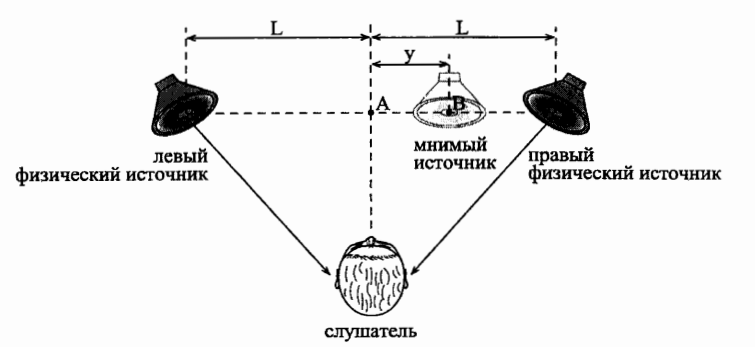
\includegraphics[width=0.8\linewidth]{pic-ear-16}}  
  \end{block}
\end{frame}

\begin{frame}
  \begin{block}{Запись звучания оркестра с помощью двух микрофонов} 
    \centering{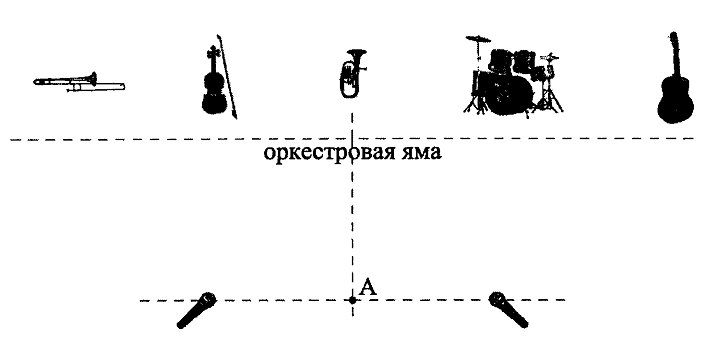
\includegraphics[width=0.6\linewidth]{pic-ear-17}}  
  \end{block}
  \begin{block}{Стереопанорама}
    воображаемая слушателем поверхность излучения звуковых волн.   
  \end{block}
Стереопанорама является частью стереобазы. Ширина стереопанорамы является максимально возможной при данном конкретном расположении физических источников звука, если она равняется ширине стереобазы (исключая специальные искусственные методы мнимого расширения стереопанорамы).
\end{frame}

\section{Музыкальный звук и шумы}
\subsection{Музыкальный звук}
\begin{frame}
  \begin{block}{Музыкальный звук}
  тональный звук, имеющий линейчатый дискретный частотный спектр. 
  \end{block}
Основные причины, относящиеся к психофизиологическим особенностям восприятия музыкального звука человеком: 
\begin{itemize}
\item инерционность слухового аппарата человека;
\item избирательность в распознавании низких и высоких частот в звуковом частотном спектре;
\item способность памяти человека лучше распознавать, усваивать и запоминать дискретную по частоте аудиоинформацию.
\item большинство музыкальных инструментов не позволяет извлекать с их помощью звуки произвольной высоты и ограничивают музыканта конкретным набором дискретных значении высоты тона.
\end{itemize}
\end{frame}

\begin{frame}
  \begin{block}{Тон в музыке}
    звук, обладающий определенной высотой звучания. 
  \end{block}  
  В современной 12-тоновой музыкальной системе различают целый тон~--- расстояние между двумя звуками, равное 1/6 октавы, и полутон~--- наименьшее расстояние между двумя звуками.
  \begin{block}{Октава}
(от лат. "<octava">~--- "<восьмая">)~--- один из музыкальных интервалов или часть музыкального звукоряда, в которую входят все звуки музыкальной системы. Высоты крайних звуков октавы различаются на слух ровно вдвое.
  \end{block}
Музыкальный звук характеризуется определенной {\itshape высотой} (от 16~Гц до 4,5~кГц), {\itshape громкостью}, {\itshape длительностью} и {\itshape тембром}. 
  \begin{block}{Высота музыкального звука}
относится к психофизиологическим параметрам, определяется каждым человеком субъективно и зависит, в основном, от частоты. 
  \end{block}
\end{frame}

\begin{frame}
  \begin{block}{Громкость звука} 
  параметр, который также связан с психофизиологией восприятия звука человеком и является мерой силы слухового ощущения интенсивности (силы звука). 
  \end{block}  
  Применительно к музыке под громкостью звука еще понимают различную относительную степень силы звучания голоса, инструмента, оркестра и т.д. В нотах громкость обозначают итальянскими терминами: {\itshape пиано} (от лат. "<piano">, сокращенно~--- Р)~--- тихо; {\itshape форте} (от лат. "<forte">~--- F)~--- громко и др.
  \begin{block}{Длительность звукового сигнала}
  временн{\'a}я характеристика звучания.  
  \end{block}
  В музыке существует ритмическое деление длительности музыкального звука на равные части. Основной вид деления~--- это деление на две части: целой ноты на две половинные, половинной ноты на две четверти, четвертной - на две восьмые и т.д., а также деление трехдольных длительностей на три части.  
\end{frame}

\begin{frame}
  \begin{block}{Музыкальная система}
  представляет собой высотную (интервальную) организацию музыкальных звуков на основе какого-либо единого принципа.   
  \end{block}

Известны музыкальные системы:
\begin{itemize}
\item из трех (трихорд~--- звукоряд из трех звуков), 
\item четырех (тетрахорд~--- 4-ступенный звукоряд), 
\item пяти (пентахорд), 
\item шести (гексахорд) 
\item семи (диатоника) 
\end{itemize} 
звуков в одной октаве.

\begin{block}{Равномерно темперированная 12-ступенная музыкальная система}
  \begin{itemize}
    \item последовательно расположены семь полных и две неполные октавы;
    \item 12 последовательных по высоте тона звуков в октаве.
  \end{itemize}
\end{block}

Все тоны на музыкальной шкале находятся в строгой математической зависимости (от лат. "<temprere">~--- "<упорядочивать">).
\end{frame}

\begin{frame}
Основой равномерно темперированной шкалы является нота "<ля"> первой октавы, имеющая частоту 440 Гц. Шкала содержит всего двенадцать полутонов и семь целых тонов (в одной октаве), обозначаемых "<до">, "<ре">, "<ми">, "<фа">, "<соль">, "<ля">, "<си">.

\centering{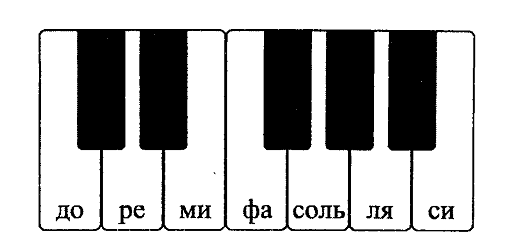
\includegraphics[scale=0.8]{pic-ear-18}}

Шкала имеет единый интервальный коэффициент для всех интервалов, равный $\sqrt[12]{2} = 1,0595$. 
\end{frame}

\begin{frame}
Изменение частоты звуковых колебаний в определенном соотношении всегда приводит к изменению высоты тона на один и тот же музыкальный интервал. Рассмотрим пример: 
\begin{itemize}
\item Для ноты $C$ первой октавы частота равна 261,6Гц. 
\item Нота $E$ выше нее~--- 329,6Гц; разница в 68Гц.
\item Нота $C$ двумя октавами ниже~--- 65,4~Гц, а $E$ выше нее~--- 82,4~Гц; только на 17~Гц выше. 
\item Нота $C$ двумя октавами выше~--- 1046,5~Гц, а $E$ выше нее~--- 1318,5~Гц; т. е. выше на 272~Гц.
\end{itemize}

Несмотря на это переход от $C$ к $E$ звучит одинаково в каждом случае. Данный интервал~--- большая терция~--- звучат одинаково в разных позициях, хотя абсолютная разница между частотами изменяется, а вот отношение частот одинаково~--- около $1:1,25$.

\begin{block}{Транспонирование}
перенесение музыкального произведения из одной тональности в другую.
\end{block} 
\end{frame}

\subsection{Шум и его разновидноси}
\begin{frame}
\begin{block}{Шум}
звук, который обладает сплошным спектром, т.е. частоты такого спектра образуют непрерывный ряд значений и целиком (без каких-либо интервалов) заполняют некоторый звуковой фрагмент.
\end{block}
Отличительная особенность шума~--- это в большинстве своем беспорядочные непериодические звуковые колебания, характеризующиеся случайными изменениями амплитуды, частоты и фазы звуковых волн, входящих в результирующую звуковую волну. 

\begin{table}
  \caption{Примеры шумов с их приблизительными уровнями громкости}
  \begin{center}
  \begin{tabular}{|l|c|}
  \hline Пример шума & Уровень громкости, дБ \\
  \hline Тихая улица без транспорта & 30-35 \\
  \hline Городская улица с транспортом & 70-80 \\  
  \hline Авторемонтная мастерская & 80-90 \\  
  \hline Кузнечный цех & 100-110 \\    
  \hline Самолет на близком расстоянии & 120-130 \\   
  \hline   
  \end{tabular}
  \end{center}  
  \label{table-noise-01}
\end{table}
\end{frame}

\begin{frame}
\begin{itemize}
\item {\itshape Белый шум} (шум Джонсона). Такой шум имеет спектр с приблизительно постоянной спектральной плотностью на всей протяженности спектра.
\item {\itshape Розовый шум}. Спектр такого шума имеет спектральную плотность, уменьшающуюся на 3 дБ с каждой последующей октавой (спектральная плотность обратно пропорциональна частоте).
\item {\itshape Оранжевый шум}. Это квазипостоянный шум с конечной спектральной плотностью. Спектр такого шума имеет полоски нулевой энергии, рассеянные на
всей его протяженности. Такие полоски находятся около частот, соответствующих музыкальным нотам.
\item {\itshape Зеленый шум}. Подобен розовому шуму с усиленной областью частот в районе 500 Гц.
\item {\itshape Синий шум}. Его спектральная плотность увеличивается на 3 дБ с каждой последующей октавой (спектральная плотность пропорциональна частоте).
\end{itemize}
\end{frame}

\begin{frame}
\begin{itemize}
\item {\itshape Фиолетовый шум}. Это дифференцированный белый шум. Его спектральная
плотность увеличивается на 6 дБ с каждой последующей октавой (спектральная плотность пропорциональна квадрату частоты).
\item {\itshape Серый шум}. Спектр такого шума имеет график, аналогичный графику психоакустической кривой порога слышимости. Это значит, что для слухового
аппарата человека этот шум имеет одинаковую громкость на всем слышимом диапазоне частот.
\item {\itshape Коричневый шум}. Его спектральная плотность уменьшается на 6 дБ с каждой последующей октавой (спектральная плотность обратно пропорциональна квадрату частоты). 
\item {\itshape Черный шум}. Определений этого шума существует достаточно много. Мы остановимся на следующем. Черным шум~--- это сверхзвуковой белый шум. Такой шум имеет постоянную конечную спектральную плотность за пределами порога слышимости (20 кГц).
\end{itemize}
\end{frame}

\begin{frame}
  \begin{block}{Спектрограмма белого шума}
    \centering{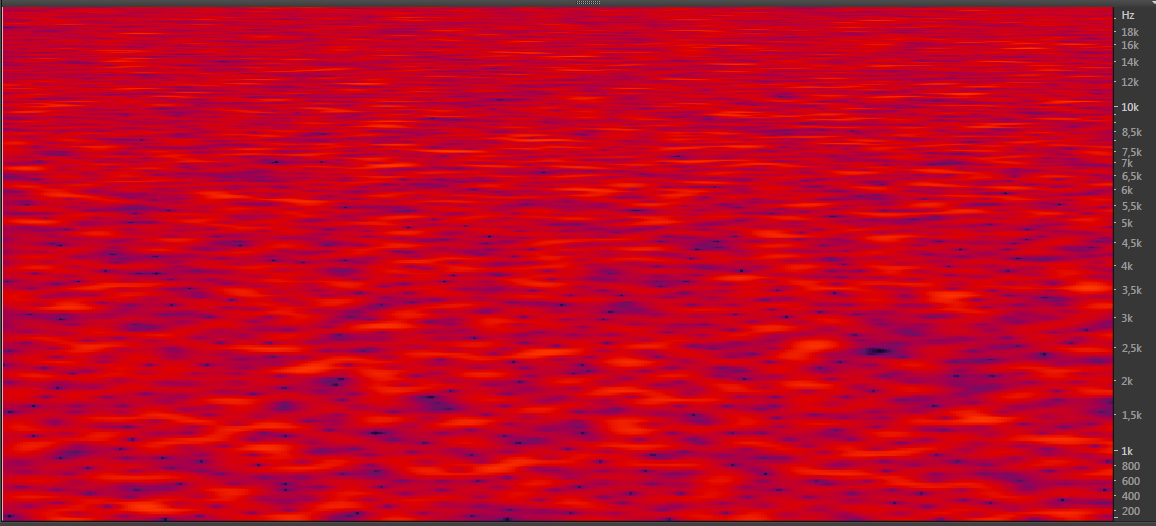
\includegraphics[width=0.9\linewidth]{pic-noise-01}}
  \end{block}
\end{frame}

\begin{frame}
  \begin{block}{Спектрограмма коричневого шума}
    \centering{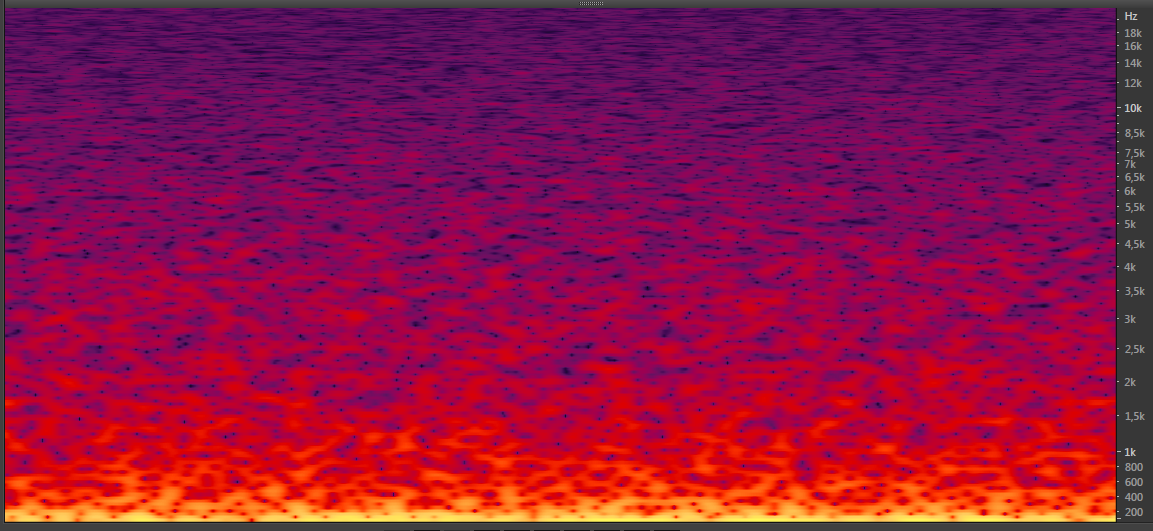
\includegraphics[width=0.9\linewidth]{pic-noise-03}}
  \end{block}
\end{frame}

\begin{frame}
  \begin{block}{Спектрограмма розового шума}
    \centering{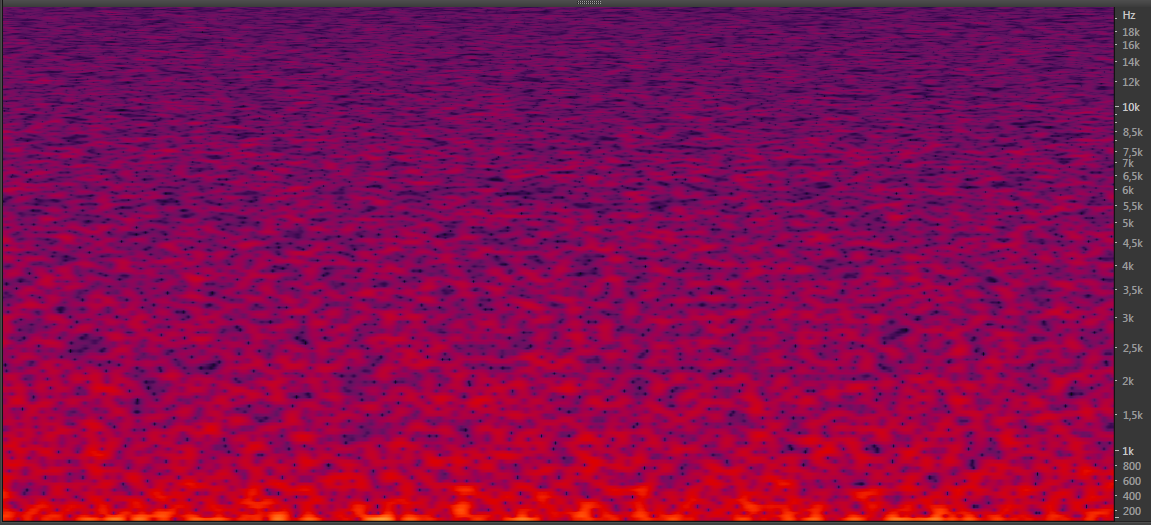
\includegraphics[width=0.9\linewidth]{pic-noise-02}}
  \end{block}
\end{frame}

\begin{frame}
  \begin{block}{Сигналограмма записи речи в малозашумленном помещении}
    \centering{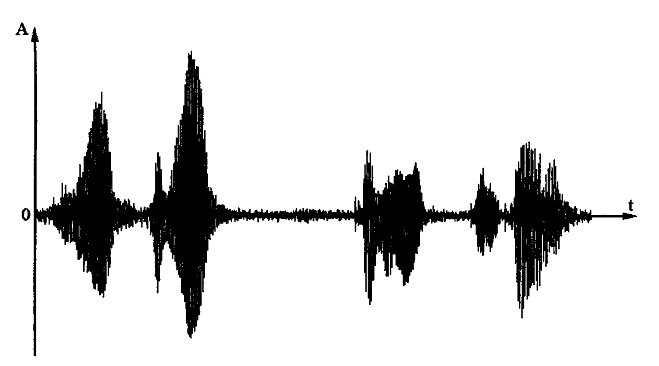
\includegraphics[width=0.9\linewidth]{pic-noise-04}}
  \end{block}
\end{frame}


\begin{frame}
  \begin{block}{Сигналограмма записи речи в зашумленном помещении}
    \centering{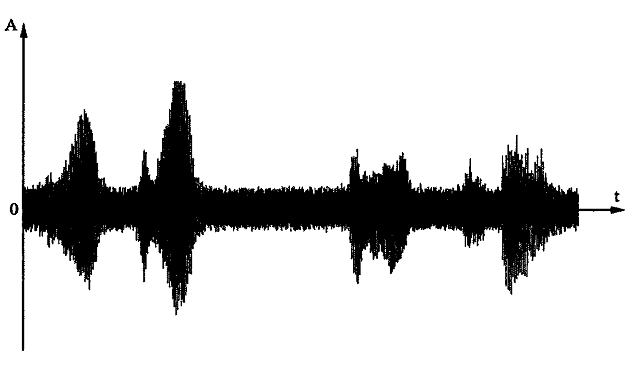
\includegraphics[width=0.9\linewidth]{pic-noise-05}}
  \end{block}
\end{frame}

\begin{frame}
Отношение Сигнал/Шум (SNR) показывает отношение уровня полезного сигнала $S$ к уровню шума $N$.
  \begin{block}{Иллюстрация отношения С/Ш}
    \centering{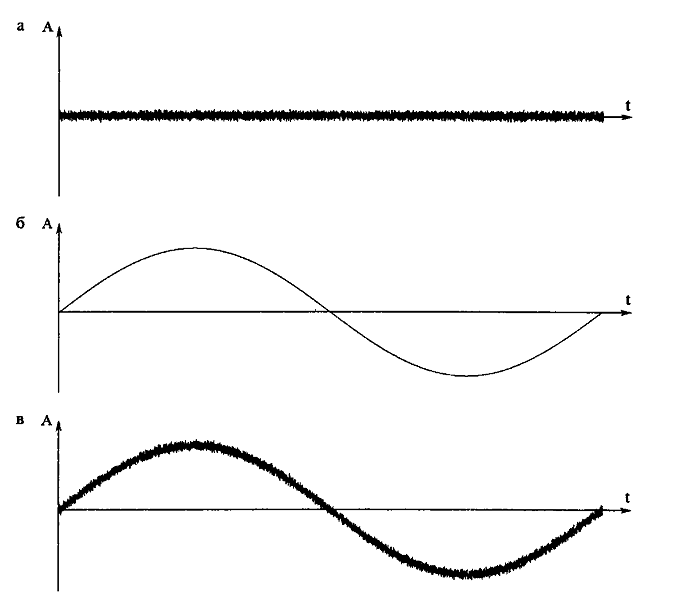
\includegraphics[width=0.5\linewidth]{pic-noise-06}}
  \end{block}
\end{frame}  
\begin{frame}  
Отношение С/Ш устройства рассчитывается по формуле
\[SNR=20 \log_{10}{\frac{S}{N}}, \text{дБ.}\]

\begin{table}
  \caption{Отношение С/Ш для некоторых типов аудиоаппаратуры}
  \begin{center}
  \begin{tabular}{|l|c|}
  \hline Тип аудиоаппаратуры & С/Ш, дБ \\
  \hline Телефонный канал & 10-20 \\
  \hline Воспроизводящая аудиоаппаратура среднего класса & 60-80 \\  
  \hline Качественная аудиоаппаратура & 80-100 \\  
  \hline
  \end{tabular}
  \end{center}  
  \label{table-noise-02}
\end{table}
\end{frame}

\end{document}
